\section{Support Vector Machines}
\smallskip \hrule height 2pt \smallskip

Vocab: 
\begin{itemize}
	\item $i$ or $j$: the $i^{th}$ or $j^{th}$ data (training) point. 
	\item $\bm{w}$: the weights of the model.  The black line is perpendicular to this vector. 
	\item $\bm{w} \cdot \bm{x}$: the distance from x to the decision boundary. 
	\item $\bm{w} \cdot \bm{x} + w_0$: to move the decision boundary off the origin, you need to shift it by a constant.  
	\item $\bm{w}_0$: a constant that defines a line parallel to the decision boundary and is $w_0$ units away. 
\end{itemize}

Like perceptron, but maximizes the margin.  

Optimizing a small weight vector: $\displaystyle min_w \: \frac{1}{2}||w||^2$ \hfill  \\  % \: gives 4/18ths of \quad space.
	% https://www.andy-roberts.net/res/writing/latex/hspacing.pdf
and getting points right: $\forall \mbox { points } i, y$  $w_{y^*} \cdot x^i \geq w_y \cdot x^i + 1$
Summary:
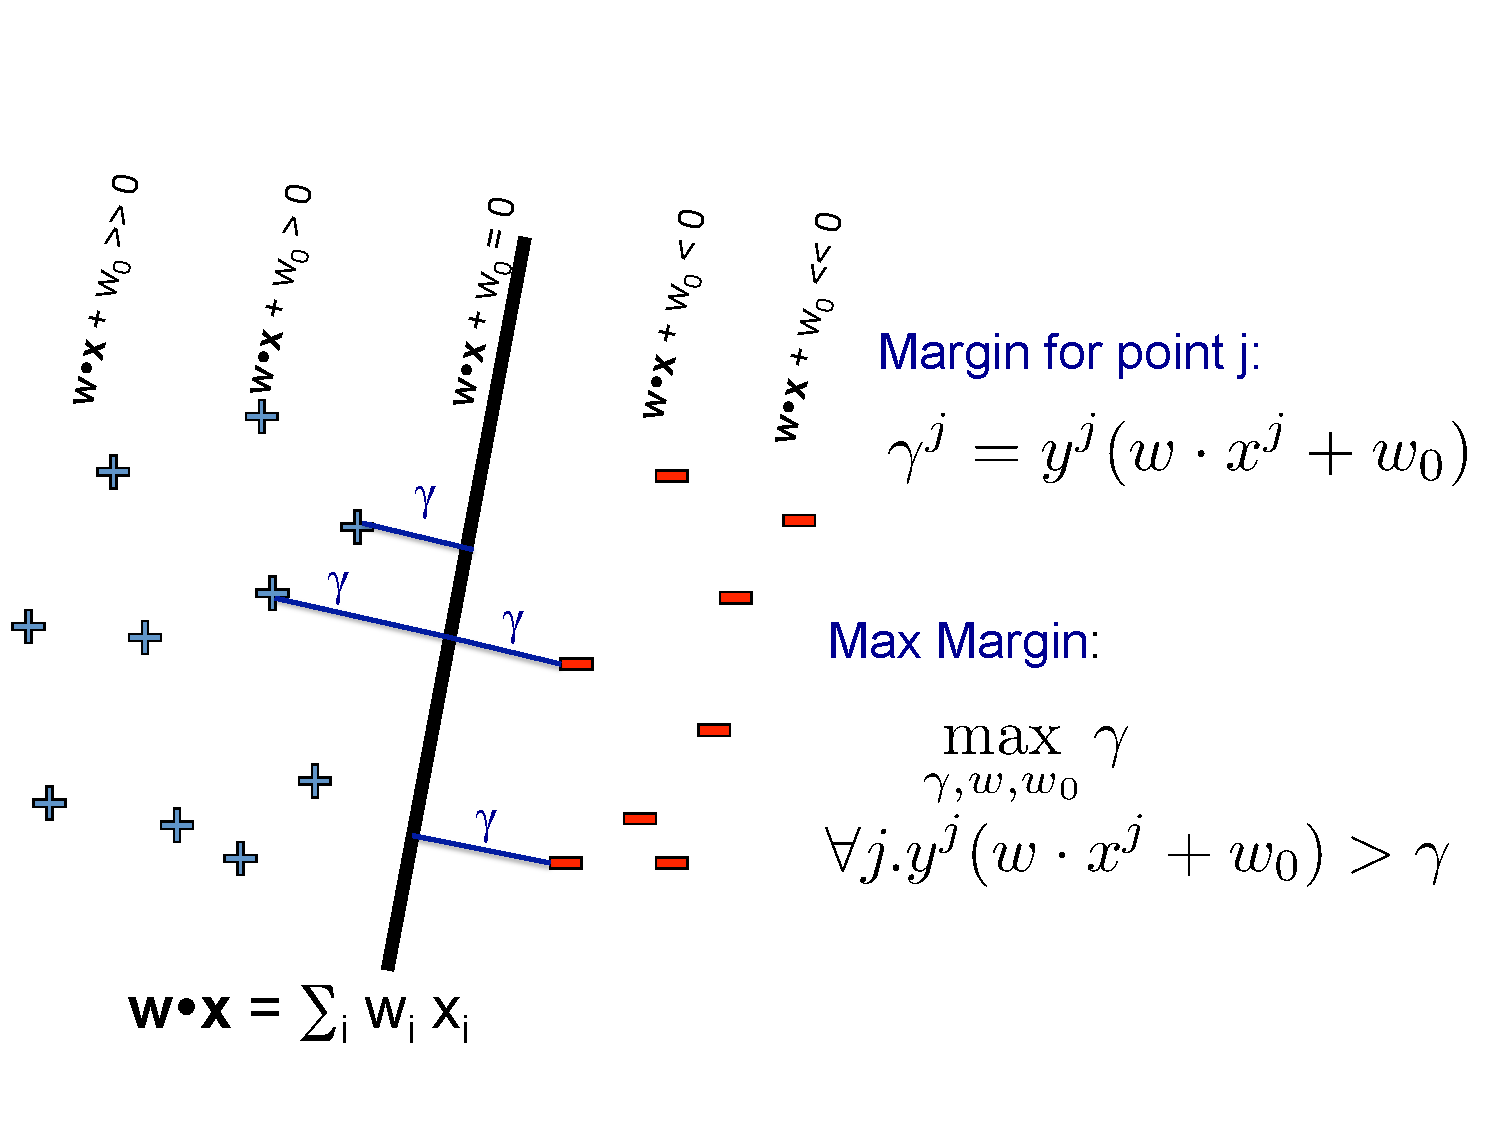
\includegraphics[width=2.5in]{figures/svm_overview.pdf}

There are many possible ways to write the same line: \hfill \\
If $\bm{w} \cdot \bm{x} + w_0 = 0$, then these also work: 
$2\bm{w} \cdot \bm{x} + 2w_0 = 0$, $1000\bm{w} \cdot \bm{x} + 1000w_0 = 0$, $\dots$ \hfill \\
Any constant scaling has the same intersection with the z = 0 plane, so you get the same dividing line. \hfill \\
\textbf{This is why we \underline{don't} want} max$_{\gamma, w, w_0}$. \hfill \\  \hfill \\

%Recall that the distance from the the decision boundary to a point is given by $\gamma$
%\includegraphics[width=2.5in]{figures/svm_dist_to_plane.pdf}

The distance from $x^j$ to the decision boundary is given by $\lambda \frac{w}{||w||_2}$ :  \hfill \\
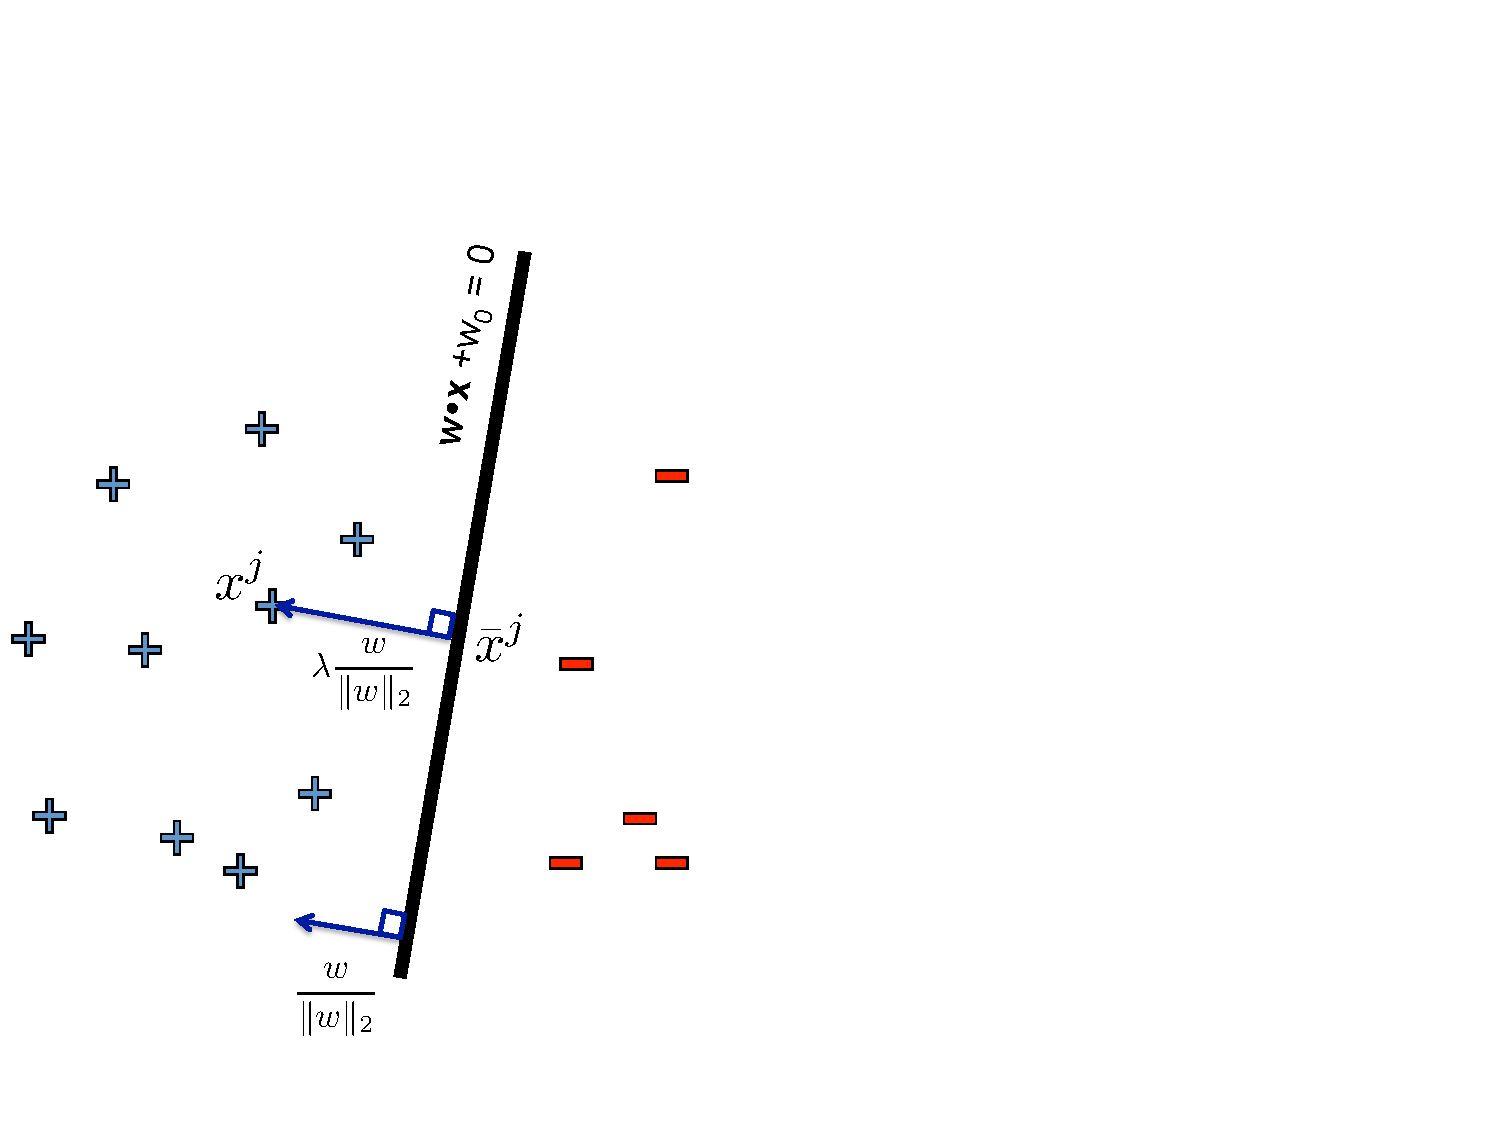
\includegraphics[width=1.5in]{figures/svm_component_norm_to_decision_boundary.pdf}  \hfill \\
$\bar{x}^j$ is the component of $x^j$ that is normal to $w$. \hfill \\
So $x^j = \bar{x}^j + \lambda \frac{w}{||w||_2}$  \hfill \\
(Recall $||w||_2 = \sqrt{\sum_i w_i^2}$)  \hfill \\   \hfill \\

\subsection{motivation for minimizing the norm of the weights}
We can maximize the margin by minimizing $||w||_2$: 
$\gamma = \frac{||w||_2}{w \cdot w} = \frac{1}{||w||_2}$   \hfill \\
Derivation:  \hfill \\
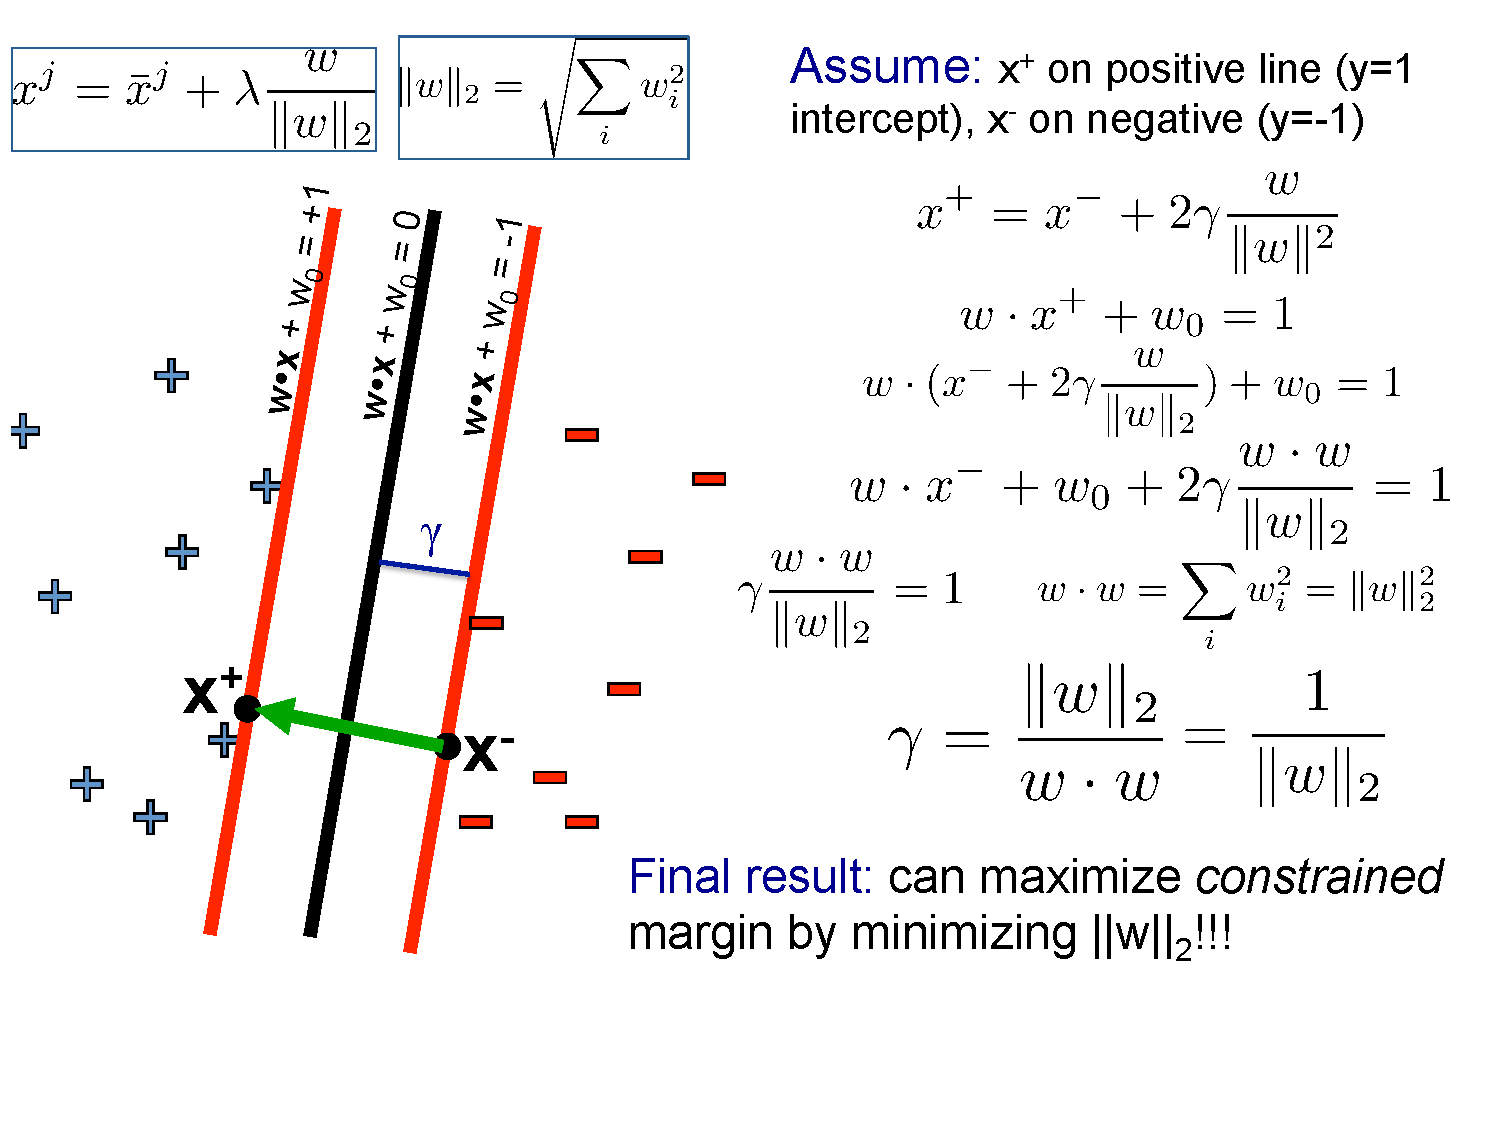
\includegraphics[width=2.7in]{figures/svm_derivation_of_minimizing_weights.pdf} \hfill \\

Intuitive explanation, after 2 key facts:  \hfill \\
\begin{itemize}
	\item Key fact \#1: the bigger your $\bm{w}$ is, the \underline{closer} the line $\bm{w}\bm{x}=1$ is to the line $\bm{w}\bm{x} = 0$.  		Small distance between $\bm{w}\bm{x}=1$ and $\bm{w}\bm{x}=0$ translates to a small margin.  
		Note that you could use any constant in place of 1. 
	\item Key fact \#2: The $w_0$ just shifts the black decision boundary line away from the origin.  
\end{itemize}
Now we can explain why minimizing the norm of the weights leads to the largest margin. 

\begin{itemize}
	\item Imagine $w_0 = 0$, meaning the decision boundary goes through the origin.  \hfill \\
	\item Now let $w = [2, 0]$ for simplicity.    
		Where is the decision boundary?  
		The decision boundary corresponds to $2 x_0 + 0 x_1 = 0$.  
		That means the decision boundary is along $x_0 = 0$, which is a line through the $x_1$ (vertical) axis. 
	\item But the point is that when you set $\bm{w} \cdot \bm{x} = c$ or some other constant.
		Key fact \#1 says that the larger w is, the farther $\bm{w} \cdot \bm{x} = 0$ is from $\bm{w} \cdot \bm{x} = c$  
		In this case where $w_1 = 0$, you have  $w_0 x_0 = c$, or $x_0 = c/w_0 = c/2$.  
		If you want the $=1$ line far from the decision boundary, you need to increase the distance between these lines.
		Since $c$ is fixed, so the only way we can do this is to decrease $w_0$. 
	\item The logic holds true for when $w_1$ is nonzero: you just want to minimize the size of the $\bm{w}$ vector.
		Minimizing the size of $w$ is equivalent to minimizing $||w||_2$ 
\end{itemize}

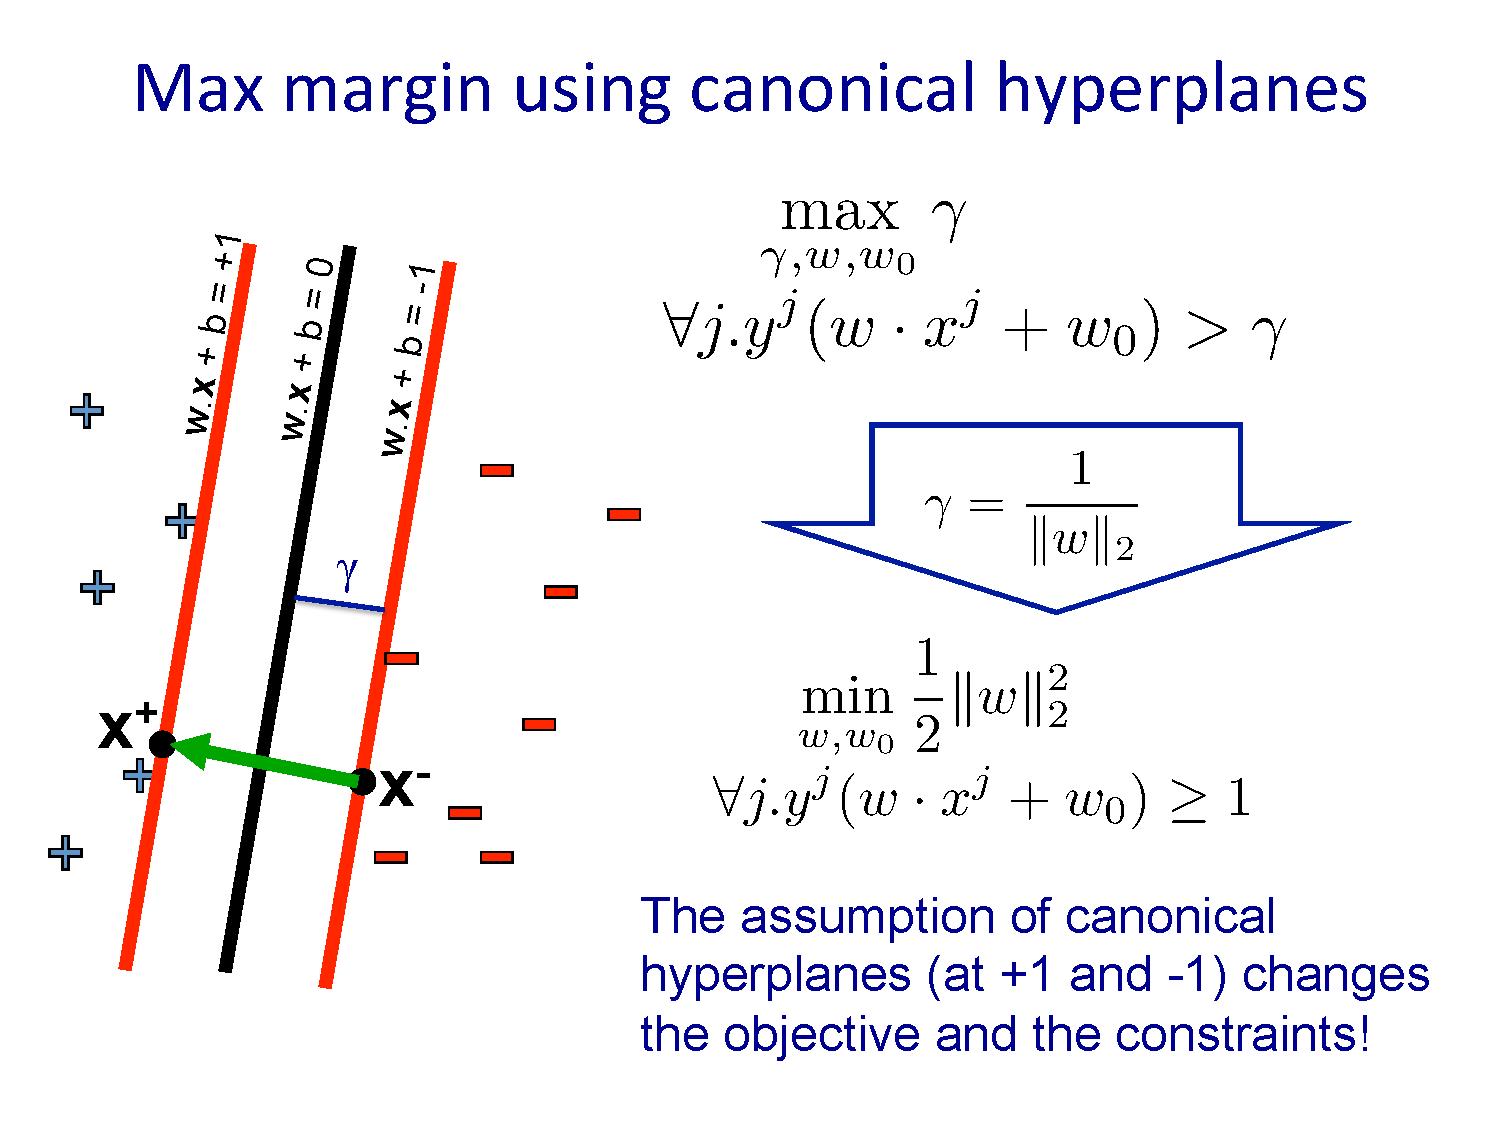
\includegraphics[width=2.7in]{figures/max_margin_using_canonical_hyperplanes.pdf}

\subsection{SVM recipe}
We want to minimize the norm subject to getting the predictions right:  \hfill \\
$\displaystyle  \min_{w, w_0} \frac{1}{2} ||w||_2^2$ so that $\forall j . y^j(w \cdot x^j + w_0) \geq 1$

We do this with quadratic programming (QP). 
The decision boundary is defined by \textbf{support vectors}, which are data points on the canonical red lines. 
All the points that aren't on the red line are non-support vectors. \hfill \\
 \hfill \\
 If your data is not linearly separable, you can add nonlinear features.
 These are called Kernels, and will be discussed later. 
 
 \subsection{Balancing \# of mistakes and $||w||_2^2$}
 If your data isn't linearly separable, then you might need to allow your $||w||_2$ to be a little bigger and make a few mistakes. 
One option: 
 $\displaystyle  \min_{w, w_0} \frac{1}{2} ||w||_2^2 + M$ (M = \# of mistakes)  \hfill \\
 so that $\forall j . y^j(w \cdot x^j + w_0) \geq 1$
 
 \subsubsection{Hinge Loss}
 One way to balance the number of mistakes and how big $w$ is:  
  $\displaystyle  \min_{w, w_0} \frac{1}{2} ||w||_2^2 + C \sum_j \xi^j$ \hfill \\
 so that $\forall j . y^j(w \cdot x^j + w_0) \geq 1 - \xi^j$ \hfill \\
 C = strength of penalty. \hfill \\
 $\xi$ is size of error for each error.  If the point is classified correctly, $\xi$ is zero.   \hfill \\
 When we want the dot product \& shift $\geq 1 - \xi^j$, the 1 is for the green-line margin, and you are wrong by $\xi$  amount. \hfill \\
 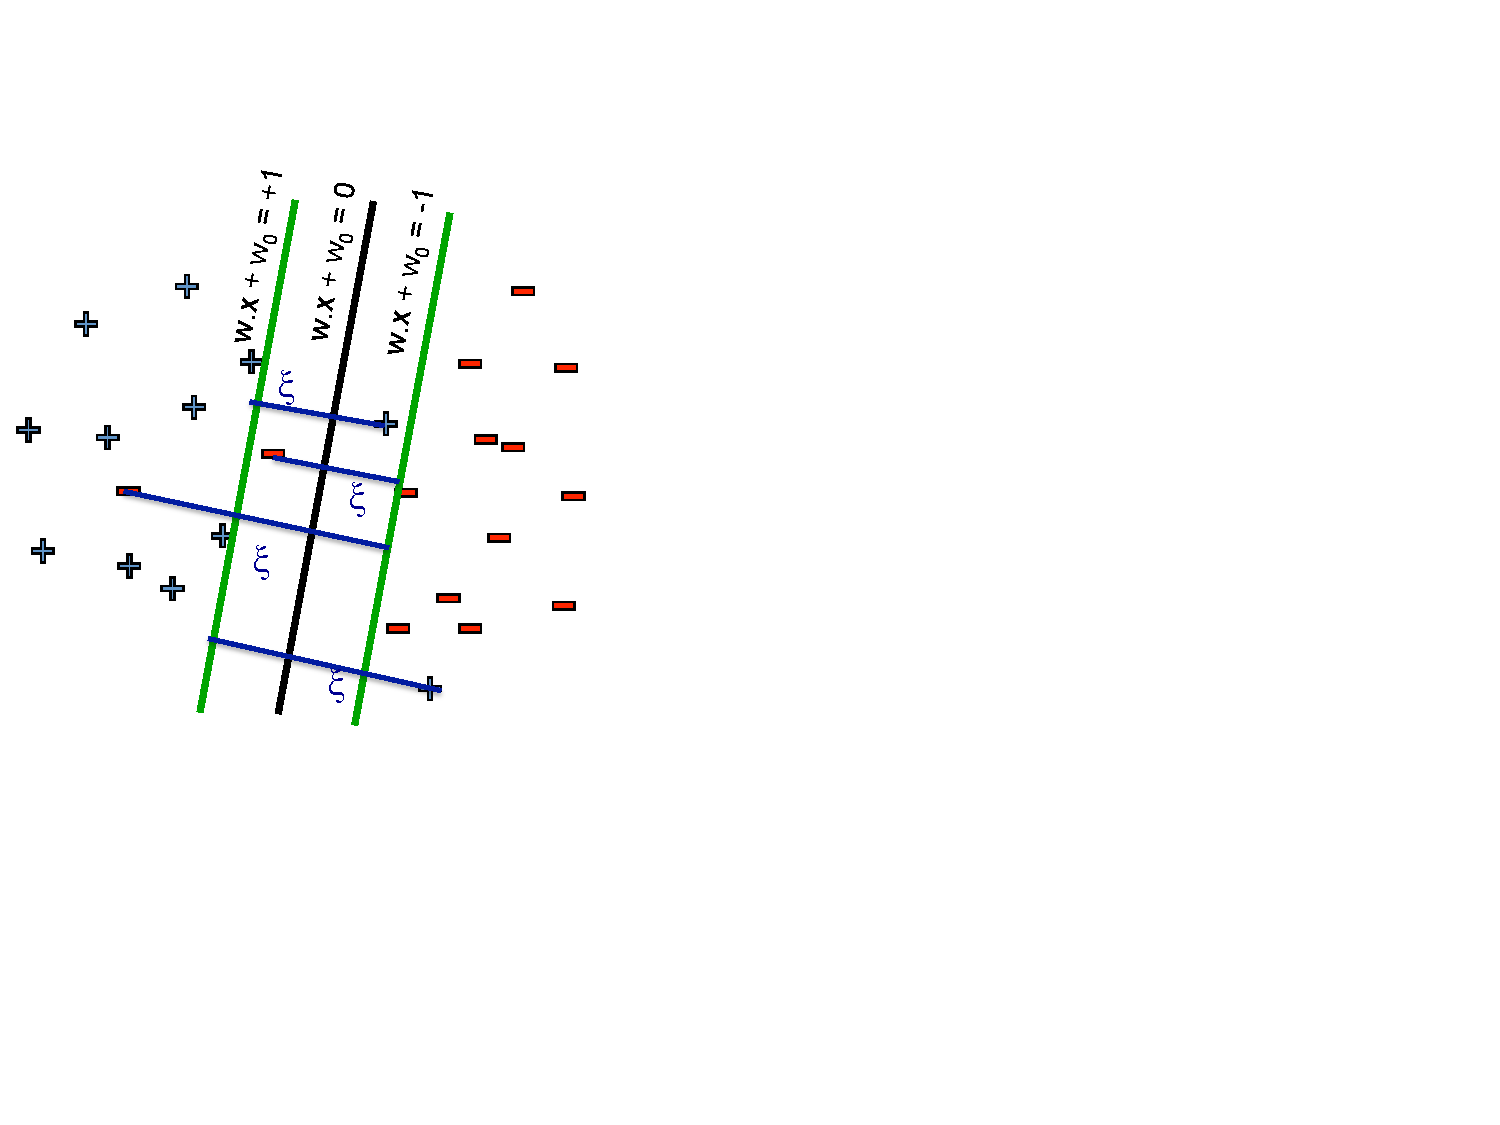
\includegraphics[width=1.5in]{figures/hinge_loss_xis.pdf}
 \hfill \\
 Now we can tune our balance between asking for small weights $\bm{w}$ and asking for perfect classification. 
 \begin{itemize} 
 	\item $C  = \infty \rightarrow$ pressure to separate the data, even if the margin is skinny.
	\item $C = 0 \rightarrow$ fat margins over accuracy. 
\end{itemize}
Use your training set to train C.  \hfill \\ 
Note that if \_\_\_\_\_ $\geq 1$, you don't care if the point is classified wrong.   % had used "margin" but this doesn't make sense!
But if \_\_\_\_\_ $ < 1$, you pay a linear penalty. % had used "margin" but this doesn't make sense! 
\hfill \\

\textbf{Hinge Loss:}  \hfill \\
$\displaystyle \min_{w, w_0} \frac{1}{2} ||w||_2^2 + C \sum_{j=1}^N [1 - y^j(w \cdot x^j + w_0)]$ \hfill \\
$1^{st}$ term is regularization, $2^{nd}$ term is hinge loss.  \hfill \\
Solve by differentiating and set equal to zero.  \hfill \\
There is no closed form solution, but quadratic program is concave.  (??)   \hfill \\
Hinge loss is not differentiable (??), so gradient ascent is a little trickier.  \hfill \\

\subsubsection{Logistic Regression to Minimize Loss}
Logistic regression assumes $P(Y=1 | X=x) = \frac{exp(f(x))}{1 + exp(f(x))}$  \hfill \\
(For Logistic Regression, $f(x)$ was $w_0 + \sum_i w_i X_i$ and we had $Y = \{0, 1\}$)  \hfill \\
Now we have $Y = \{ -1, +1 \}$.  \hfill \\
To maximize data likelihood for $Y = \{ -1, +1 \}$: \hfill \\
$\displaystyle  P(y^i | x^i) = \frac{1}{1 + exp(-y^i f(x^i))}$ \hfill \\
\begin{align*}
	\ln P(D_Y | D_{\bm{X}}, \bm{w}) &= \sum_{j=1}^N \ln P(y^j | x^j, w) \\ 
		& \mbox{plug in the $P$ above} \\
		&= - \sum_{i=1}^N \ln(1 + exp(-y^i f(x^i)))
\end{align*}
Since $-\ln(z) = \ln(1/z)$ we get to minimize this (negative):   \hfill \\
$\displaystyle  \sum_{i=1}^N \ln(1 + exp(-y^i f(x^i))) =  \sum_{i=1}^N \ln(1 + exp(-y^i [w_0 + \sum w_i x_i]))$

\subsubsection{SVMs vs Regularized Logistic Regression}
\textbf{SVM Objective:} \hfill \\
$\displaystyle \argmin_{\bm{w}, w_0} \frac{1}{2} ||w||_2^2 + C \sum_{j=1}^N [1 - y^j f(x^j)]_+$ \hfill \\
where $[x]_+ = max(x , 0)$ \hfill \\
 \hfill \\

\textbf{Logistic Regression Objective:} \hfill \\
$\displaystyle  \argmin_{\bm{w}, w_0} \lambda ||w||_2^2 + \sum_{j=1}^N ln(1 + \exp(-y^j f(x^j)))$ \hfill \\
 \hfill \\
 
 Note that SVM and Logistic Regression have the same $l_2$ regularization term, but different error terms. 

 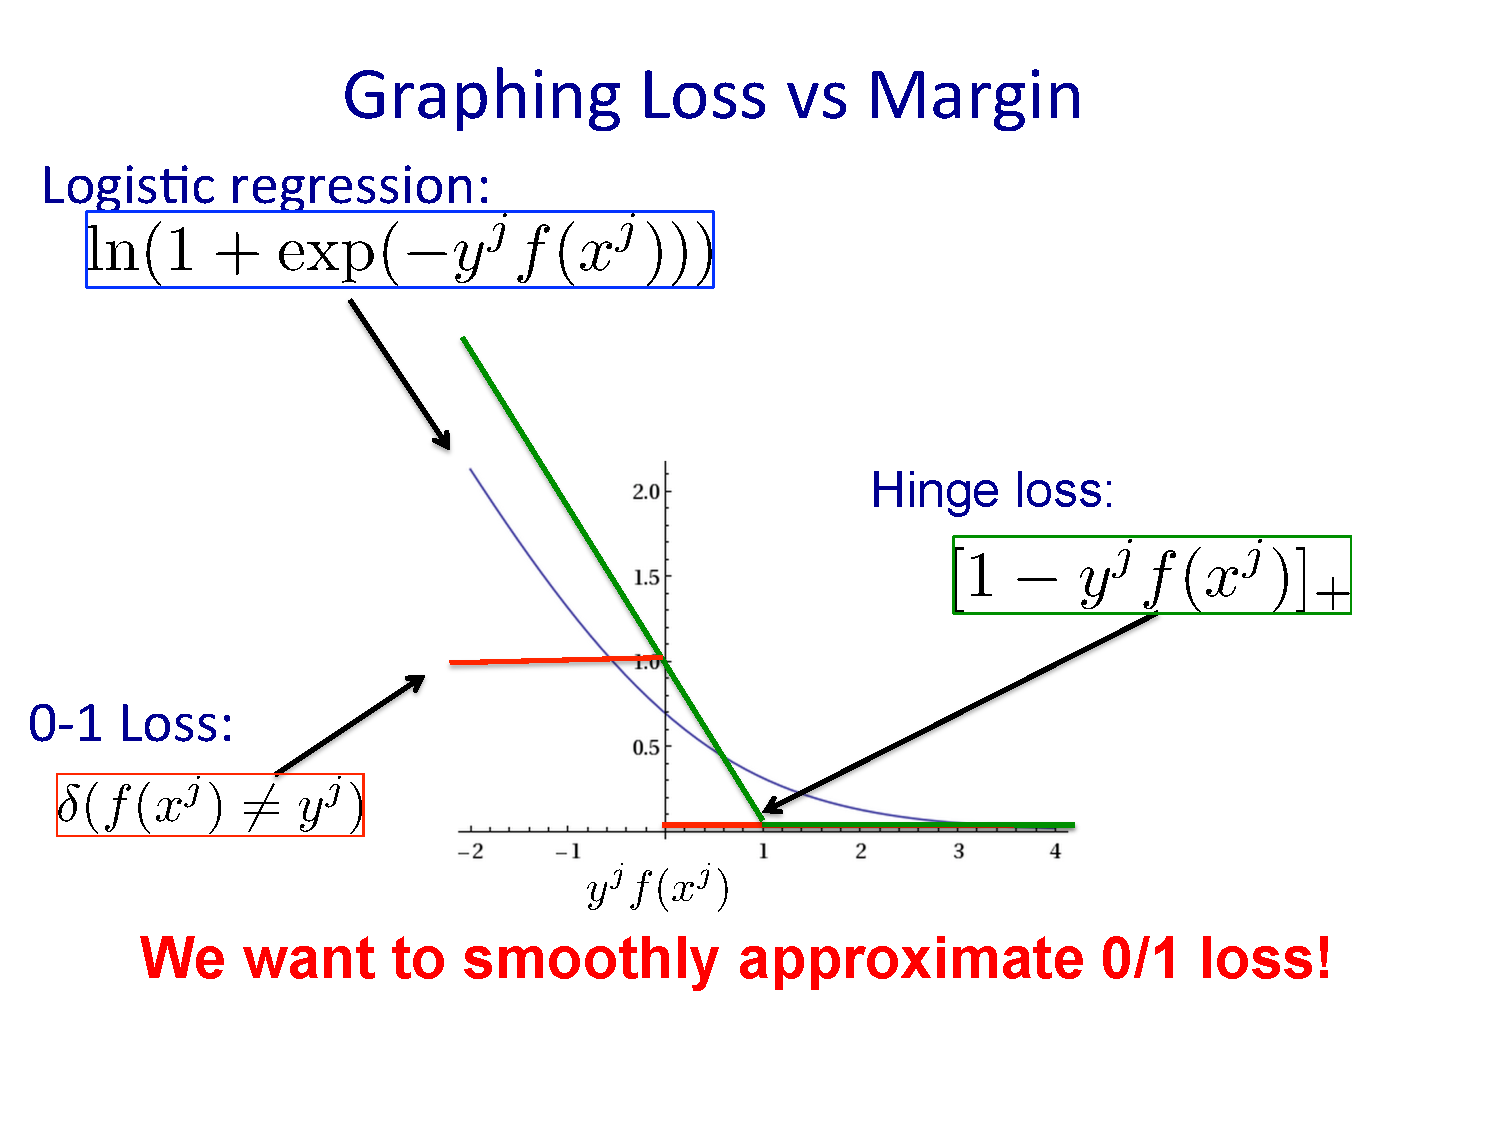
\includegraphics[width=2.5in]{figures/LR_svm_step_losses.pdf}
 
 \subsection{Multi-class SVMs}
 To do 3 classes, you need to learn 3 classifiers. \hfill \\
 Can't just do $y = \argmax_i w_i \cdot x$ for $i$ classifiers.  
 Wouldn't handle this: 
 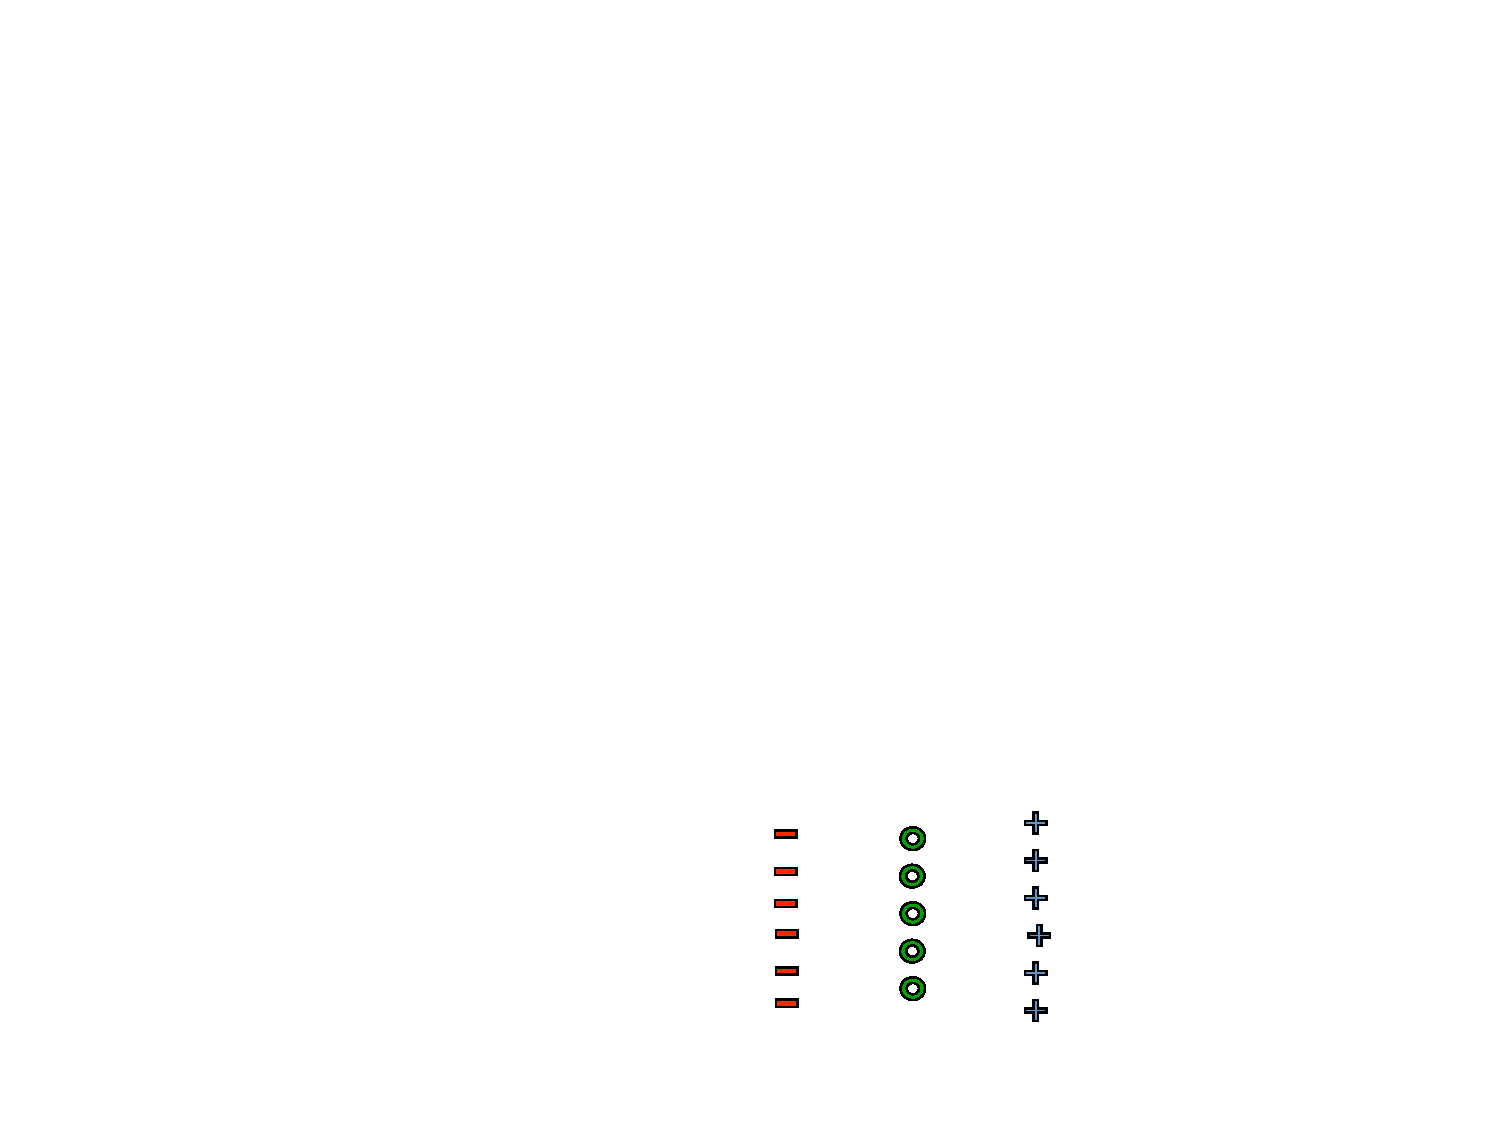
\includegraphics[width=0.6in]{figures/multiclass_svm_motivation.pdf}
 \hfill \\  \hfill \\
 
 Instead, we learn 3 classifiers for these 3 symbols: 
 \begin{enumerate}
 	\item + vs $\{ O, - \}$, weights $w_+$
	\item + vs $\{ O, + \}$, weights $w_-$
	\item + vs $\{ +, - \}$, weights $w_O$
 \end{enumerate}
 But to get it working for that set of 3 columns, we need additional constraints.  \hfill \\
 For each class: \hfill \\
 for class $y'$ that is not class $y^j$ ($\forall y' \neq y^j$):  \hfill \\
 And for all classes $j$ ($\forall j$):  \hfill \\
 $w^{y^j} \cdot x^j + w_0^{y^j} \geq w^{y'} \cdot x^j + w_o^{y'} + 1$. \hfill \\
 ($\forall$ = "for all") \hfill \\
 In plain english: ????.   \hfill \\
 ??? Do I have the fact that j is for classes right?  (Could j still be points?)  ??
 \hfill \\
 \hfill \\
 
We can also introduce slack variables as before. 
$\displaystyle \min_{w, w_0} \sum_y ||w^y||_2^2 + C \sum_j \xi^j$ \hfill \\
$w^{y^j} \cdot x^j + w_0^{y^j} \geq w^{y'} \cdot x^j + w_o^{y'} + 1 - \xi^j$. \hfill \\
That's true for class $y'$ that is not class $y^j$ ($\forall y' \neq y^j$), and all classes $j$ ($\forall j$) and for all $\xi^j > 0$ \hfill \\
 \hfill \\
 
 So you can do multiple classes in a one against all approach *or* a multiclass SVM approach.  
 

 
  



